\chapter{Results and Discussion}

This chapter presents the experimental evaluation of RayCastED across the research objectives outlined in Chapter~1. 
The experiments are designed to assess both detection accuracy and computational efficiency, covering the RayCast
representation fidelity, full benchmarking against state-of-the-art methods, cross-dataset generalization, and edge
deployment feasibility.

\section{Performance Evaluation}
\label{sec:performance-evaluation}

We first validate the RayCast representation itself, then benchmark RayCastED against prior methods, and finally
test generalization to unseen datasets.

\subsection{RayCast Representation Validation}
\label{sec:raycast-validation}

To assess how faithfully the ray-cast polygon approximates the ground truth mask, we compute the mask IoU between
the original segmentation and the polygon reconstructed from $R$ equally-spaced rays. Table~\ref{tab:raycast-iou}
reports the per-tissue IoU for $R \in \{8, 16, 32, 64\}$ across the five organ types in PanNuke.

\begin{table}[H]
	\centering
	\caption{Summary statistics of the mask IoU between ground truth nuclei and the ray-cast polygon approximation at varying numbers of rays $R$ (mean, standard deviation, median, minimum, and maximum IoU computed over 1{,}849 nuclei from the PanNuke validation set).}
	\label{tab:raycast-iou}
	\begin{tabular*}{\textwidth}{@{\extracolsep{\fill}}lcccc}
		\hline
		\textbf{Statistic} & \textbf{$R = 8$} & \textbf{$R = 16$} & \textbf{$R = 32$} & \textbf{$R = 64$} \\
		\hline
		Mean   & 0.8099 & 0.8810 & 0.9009 & 0.9078 \\
		STD    & 0.0957 & 0.0901 & 0.0795 & 0.0775 \\
		Median & 0.8425 & 0.9060 & 0.9195 & 0.9246 \\
		Min    & 0.2727 & 0.2727 & 0.2667 & 0.2667 \\
		Max    & 0.9224 & 0.9764 & 0.9843 & 0.9902 \\
		\hline
	\end{tabular*}
\end{table}


As expected, increasing $R$ produces tighter approximations. The gain from $R=16$ to $R=32$ (Mean IoU $+0.0199$, Max $+0.0205$) is substantial, while the further increase to $R=64$ yields only incremental improvement (Mean $+0.0069$, Max $+0.0034$), indicating diminishing returns beyond 32 rays. Although $R=32$ offers the best efficiency--accuracy trade-off, $R=64$ is used as the default in all subsequent experiments to maximize boundary fidelity without a significant computational penalty.

\begin{figure}[H]
	\centering
	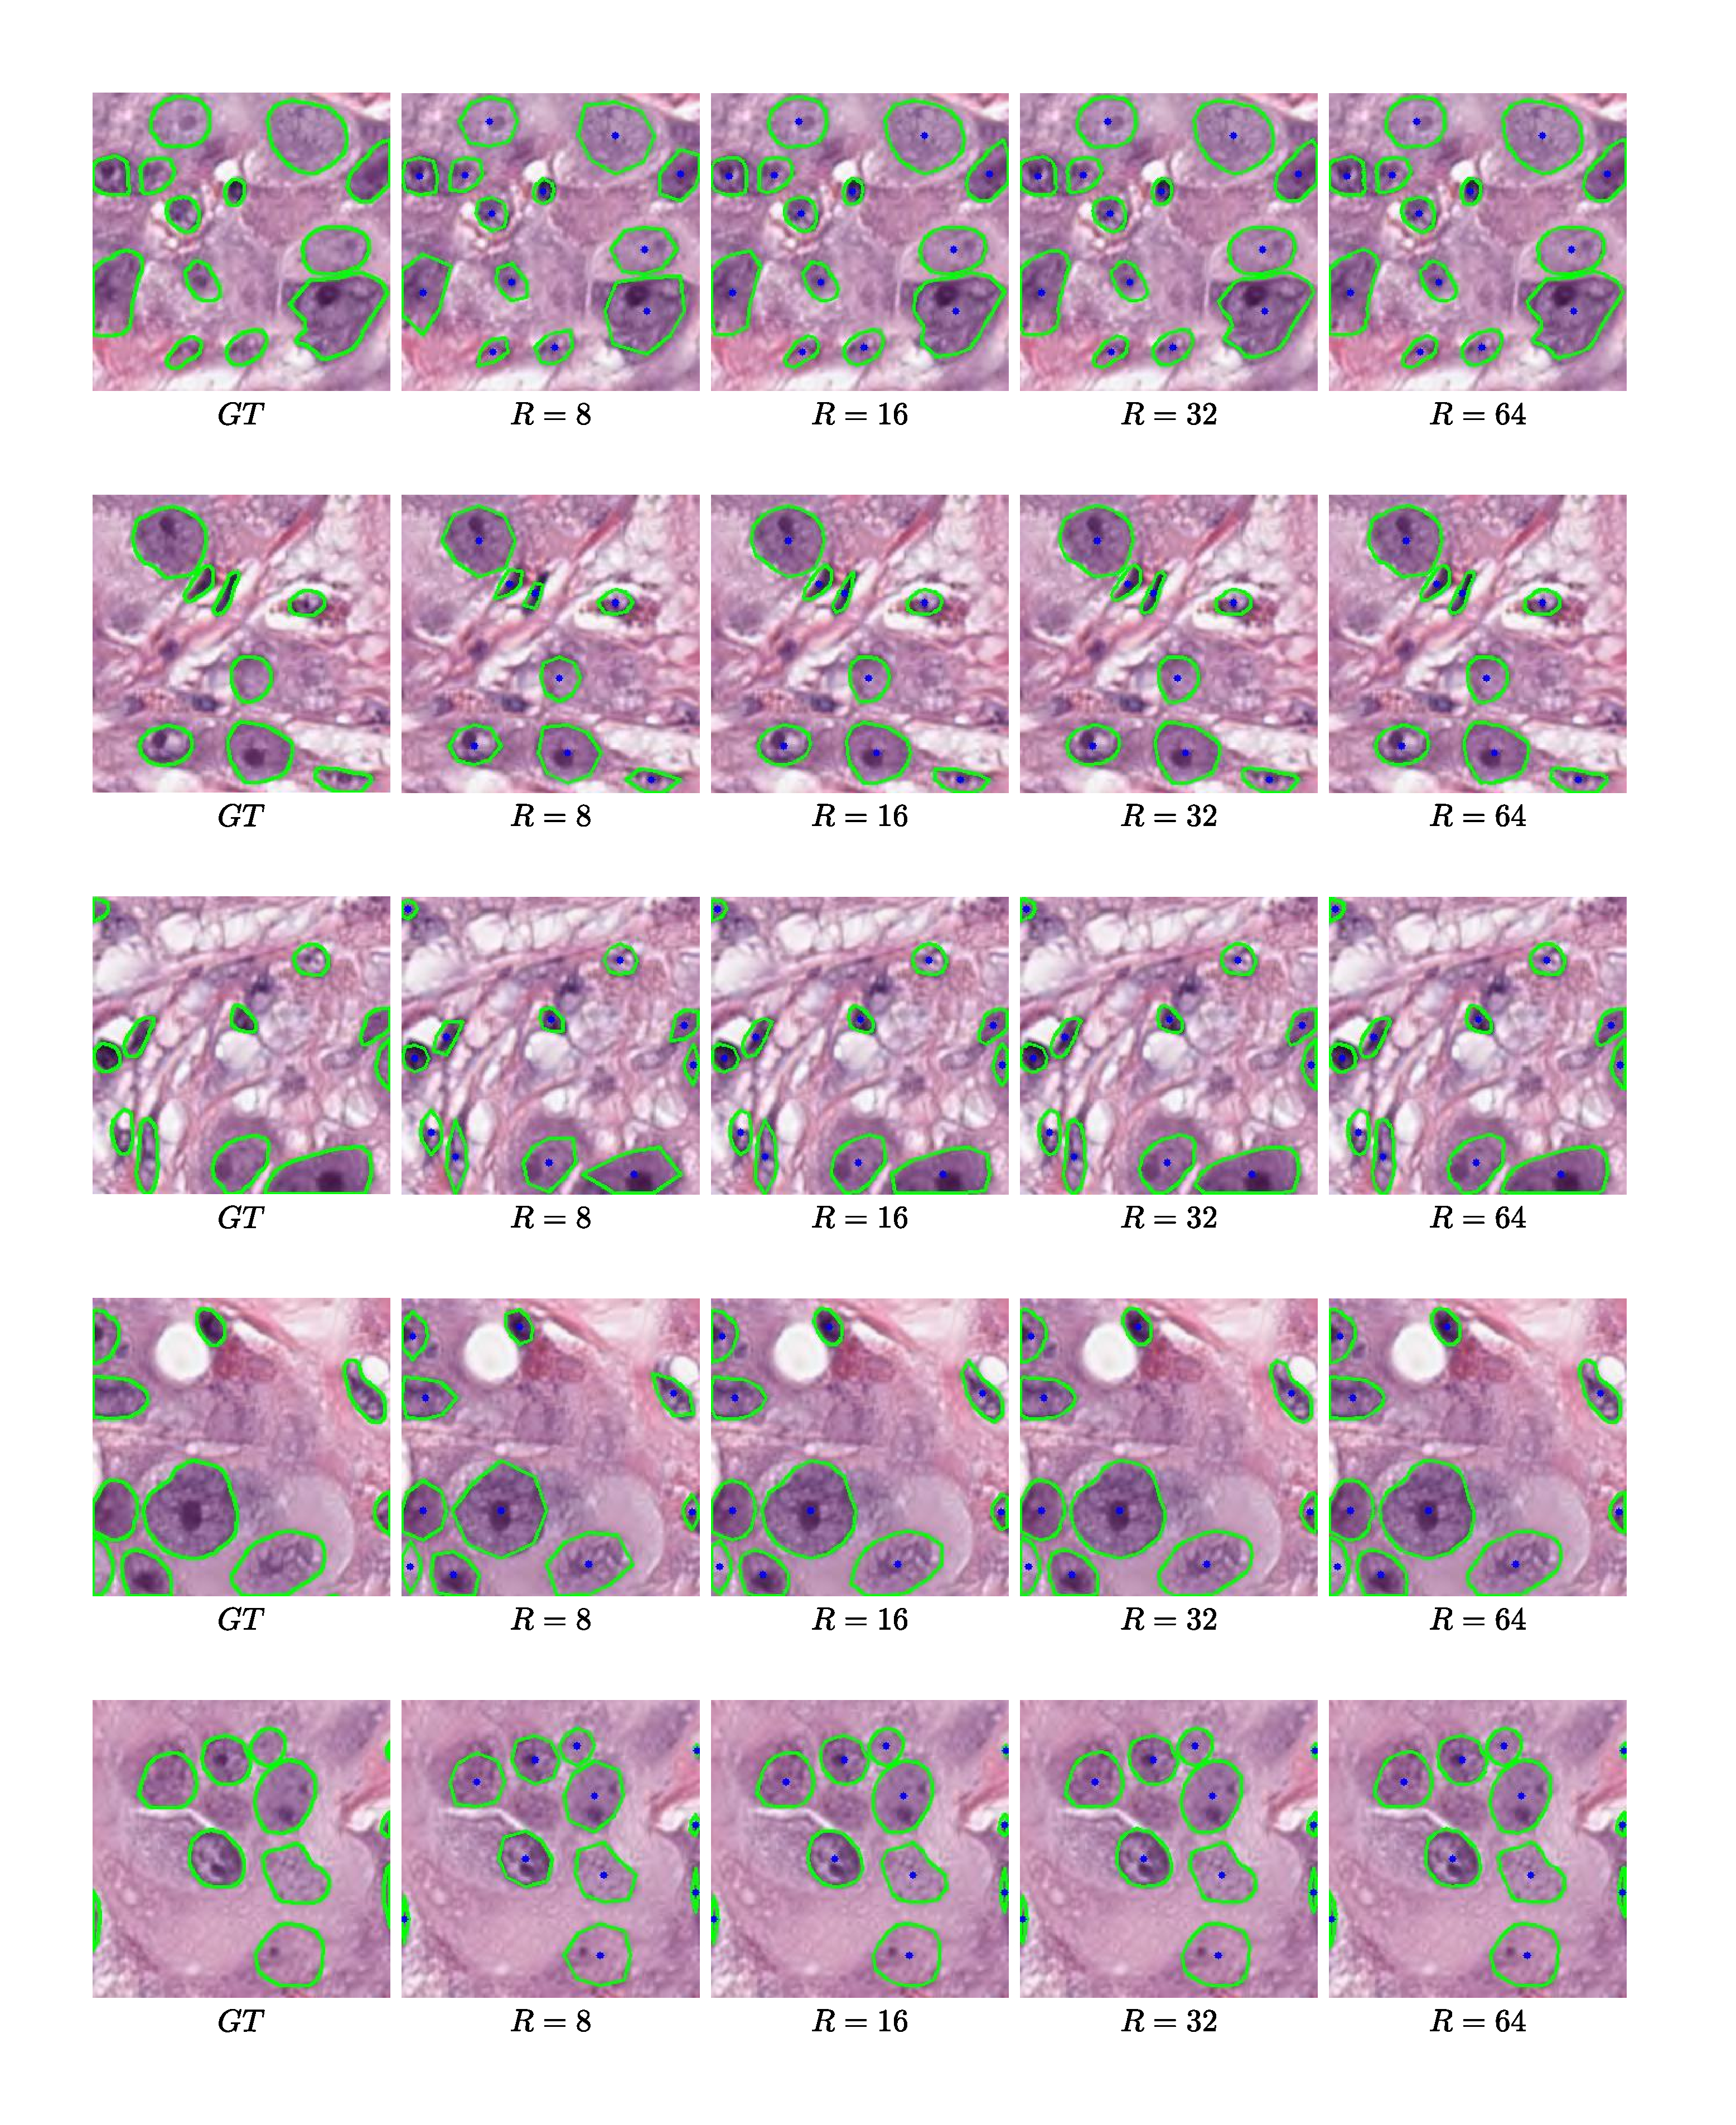
\includegraphics[width=\textwidth]{contents/chapter-4/fig/Ray_val.pdf}
	\caption{Visual comparison of ground truth nucleus mask and ray-cast polygon reconstruction at $R=8, 16, 32, 64$.}
	\label{fig:raycast-visual}
\end{figure}

\newpage
\subsection{Training Convergence}
\label{sec:training-convergence}

Before reporting final benchmark numbers, we examine RayCastED's training dynamics to confirm that the curriculum and loss schedules described in Section~\ref{sec:curriculum} produce stable convergence across all components.

Figure~\ref{fig:loss-curves} shows the five individual loss terms ($\mathcal{L}_{\text{cls}}, \mathcal{L}_{\text{xy}}, \mathcal{L}_{\text{L1}}, \mathcal{L}_{\text{piou}}, \mathcal{L}_{\text{smooth}}$) over the course of training. Because the loss weights span several orders of magnitude (e.g., $\lambda_{\text{xy}} = 500$ vs.\ $\lambda_{\text{cls}} = 2$), the curves are plotted as independent small multiples rather than on a shared axis. All five loss terms drop sharply during the early one-to-many supervised phase. The L1 ray distance loss exhibits the smoothest descent, reflecting the stable geometric supervision provided by the analytical ray recomputation from the predicted centroid. The smoothness loss remains near zero for the first 40\% of training while its weight ramps from 0 to 3; the ramp-up effect is visible as the curve lifts off and the penalty takes effect, after which it stabilizes.

\begin{figure}[H]
	\centering
	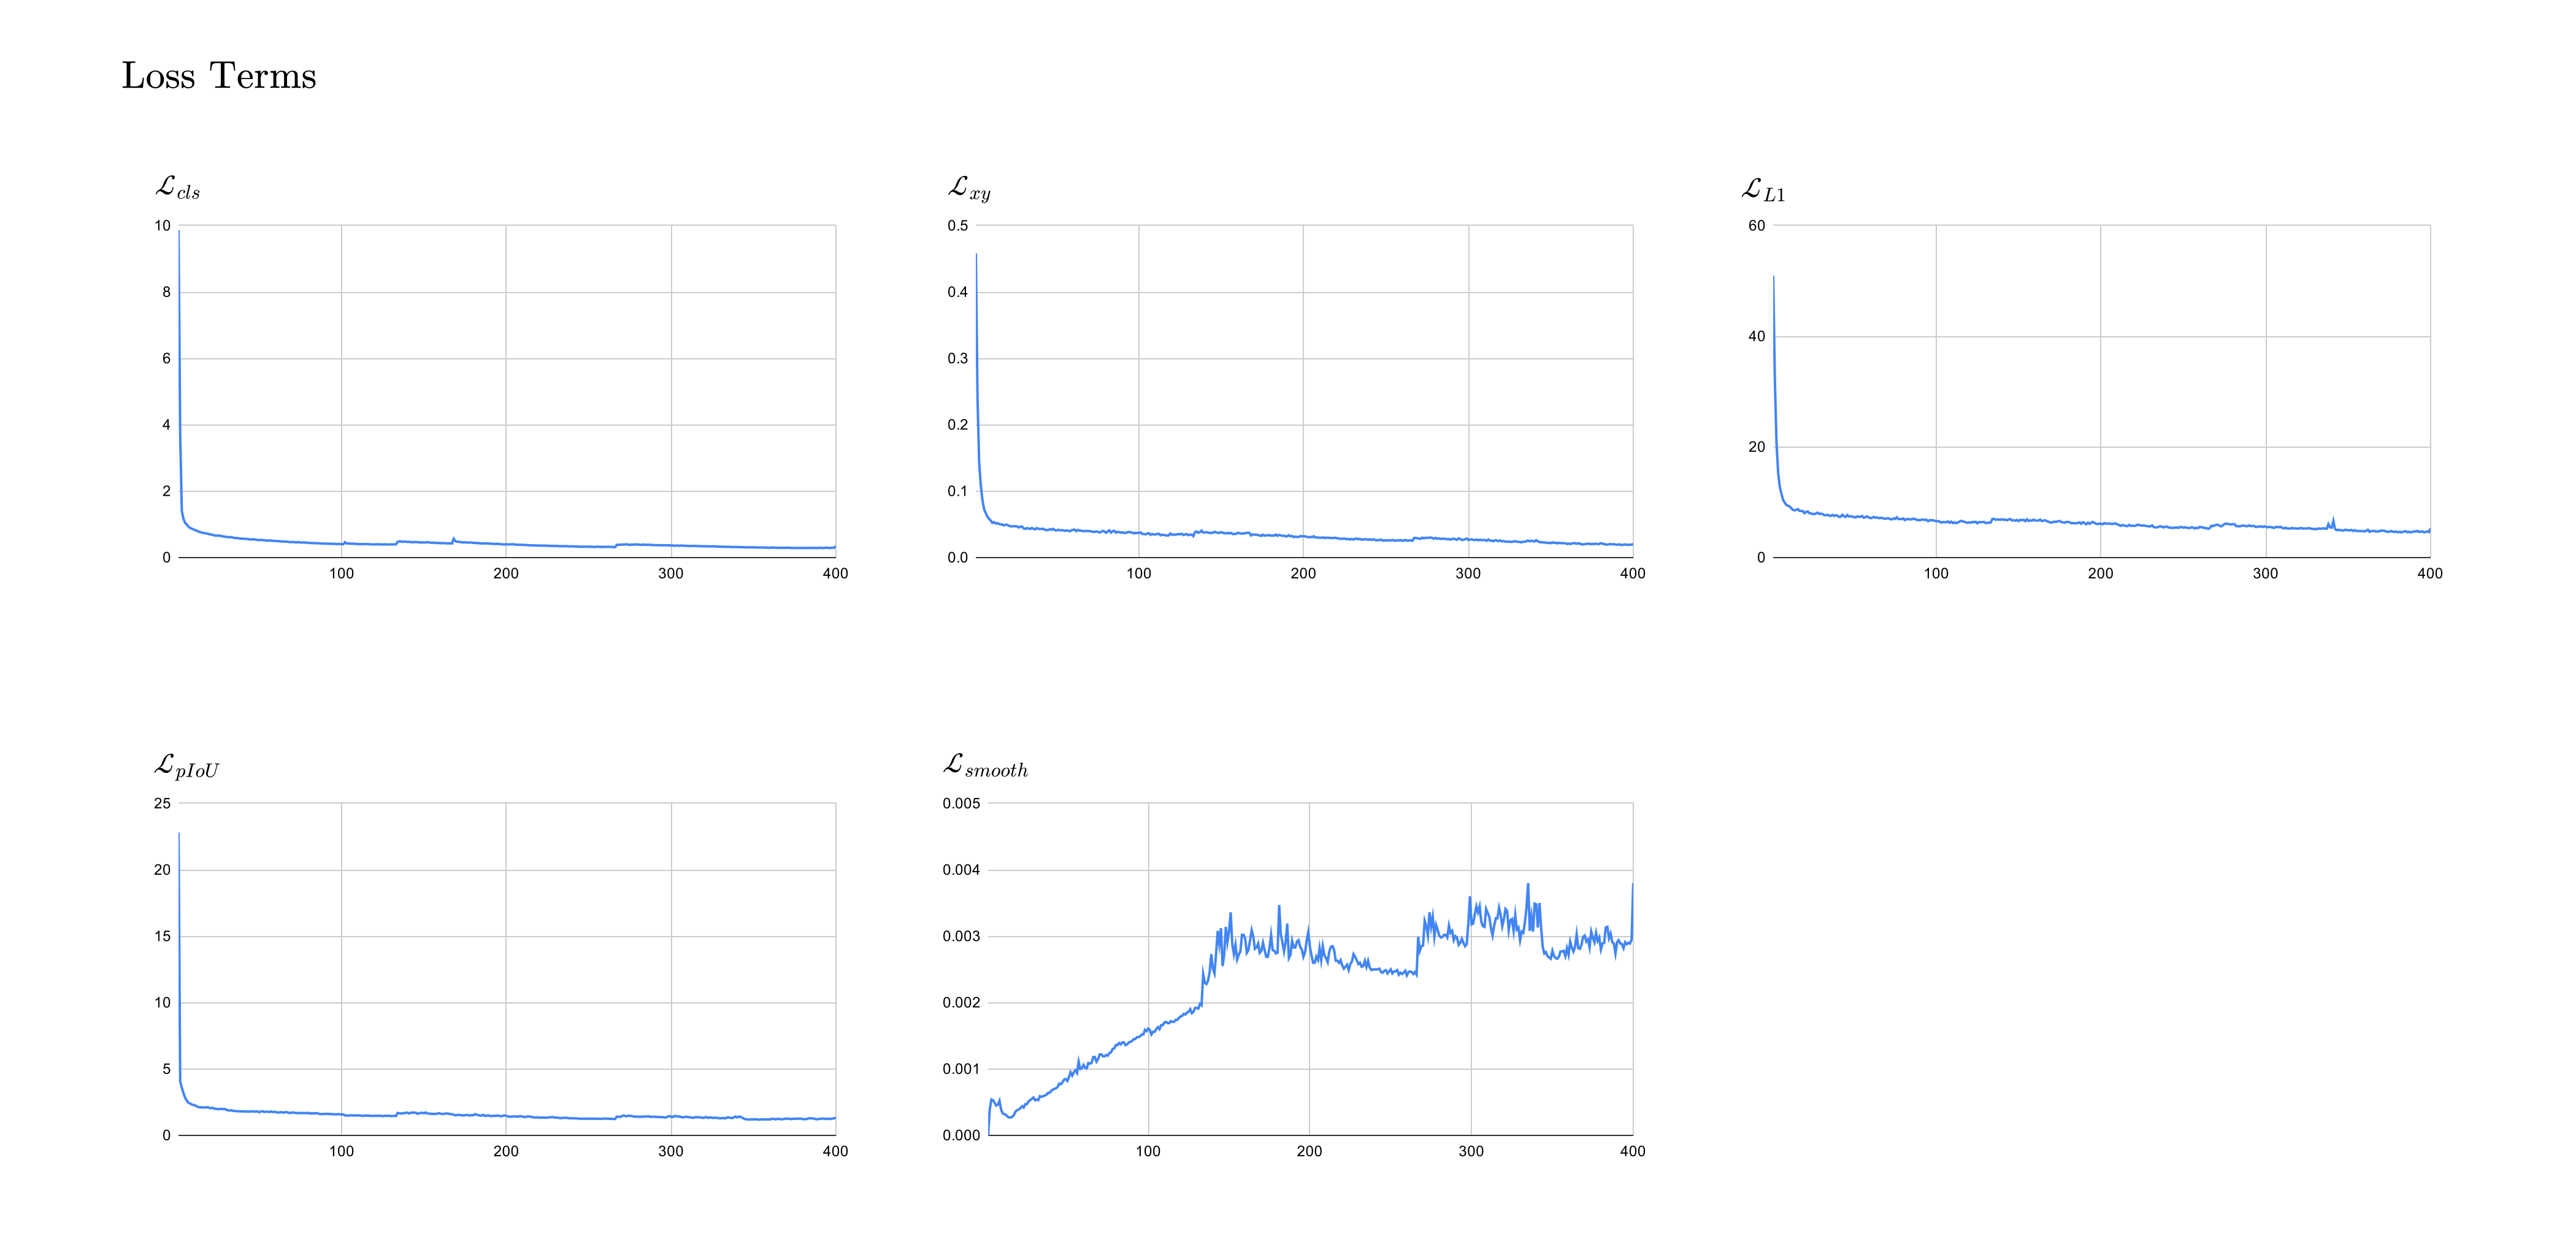
\includegraphics[width=\textwidth]{contents/chapter-4/fig/training-loss.png}
	\caption[Training loss curves for each loss term.]{Training loss curves for each loss term. Each panel shows one of the five loss components ($\mathcal{L}_{\text{cls}}, \mathcal{L}_{\text{xy}}, \mathcal{L}_{\text{L1}}, \mathcal{L}_{\text{piou}}, \mathcal{L}_{\text{smooth}}$) over the full training schedule, plotted as independent small multiples to accommodate the large range of loss magnitudes.}
	\label{fig:loss-curves}
\end{figure}

Figure~\ref{fig:metric-curves} reports the four validation metrics tracked during training: mAP$_{50}$, precision, recall, and bPQ. All four metrics improve substantially during the early training phase. Two notable rapid-climb events are visible: around epoch 100, precision and mAP$_{50}$ surge upward; and around epoch 168, precision, mAP$_{50}$, and bPQ all climb rapidly together. These jumps align with the cosine annealing restart points, where the learning rate reset allows the optimizer to escape plateau regions and refine the detection and segmentation heads further.

\begin{figure}[H]
	\centering
	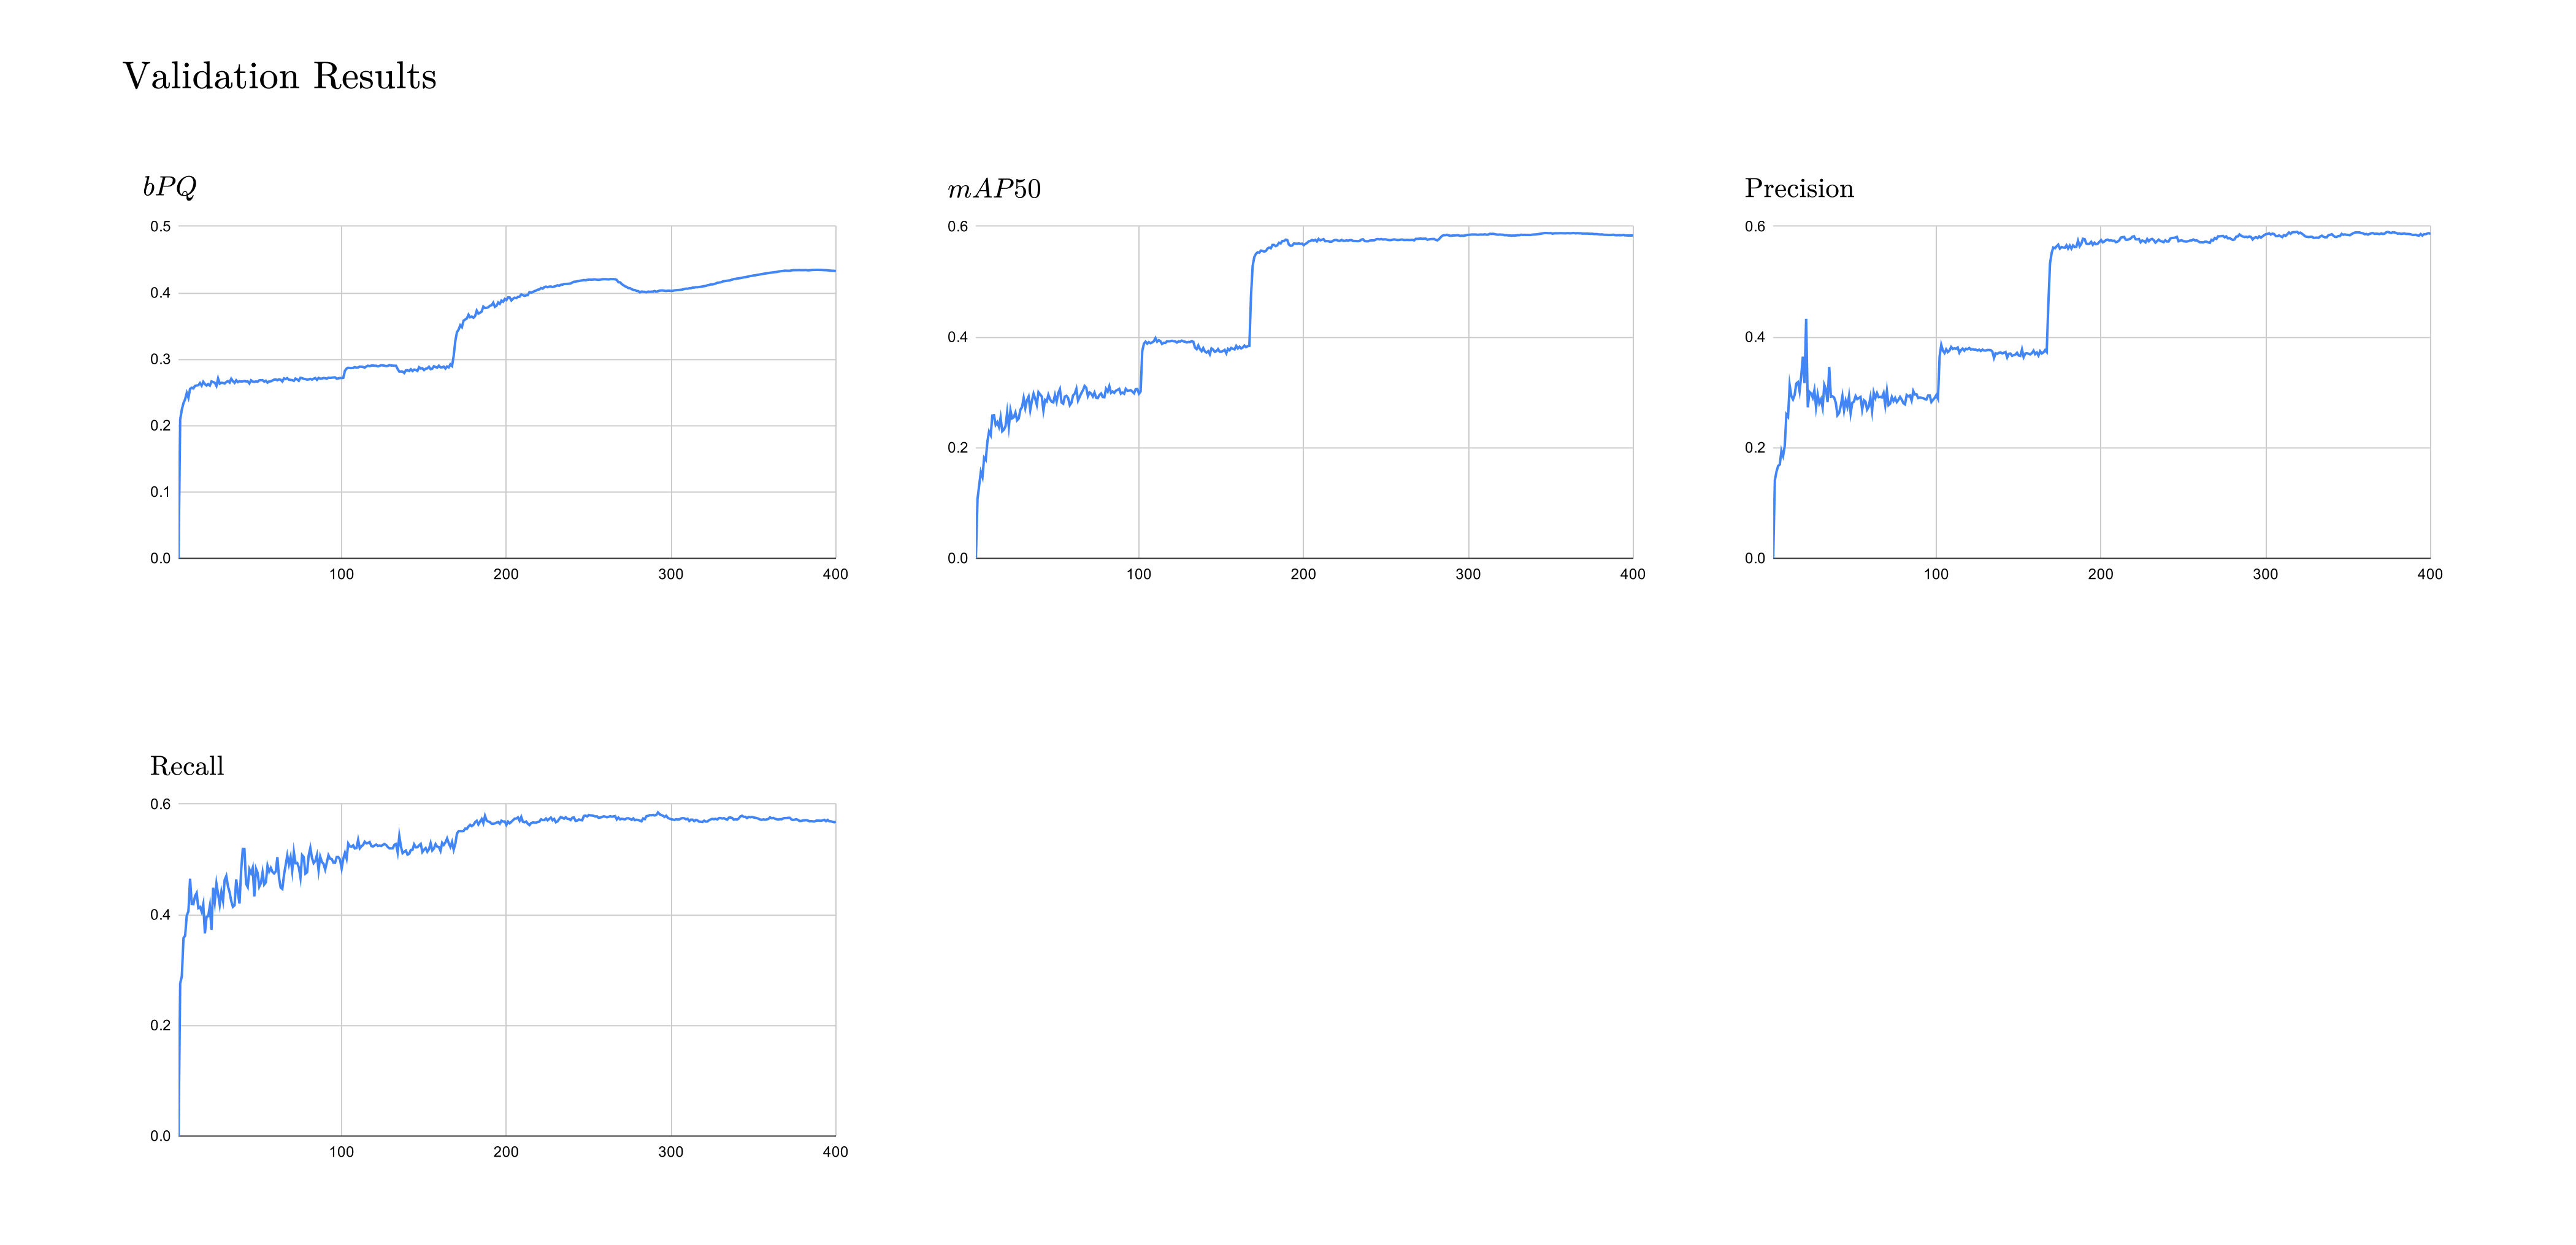
\includegraphics[width=\textwidth]{contents/chapter-4/fig/training-val.png}
	\caption[Validation metrics during training.]{Validation metrics during training. Each panel shows one of the four tracked metrics (mAP$_{50}$, precision, recall, bPQ) computed on the held-out validation fold across the full training schedule.}
	\label{fig:metric-curves}
\end{figure}

\newpage
\subsection{RayCastED Benchmarking Results}
\label{sec:benchmarking}

We compare RayCastED against five prior methods -- StarDist, CPP-Net, CellViT, LKCell, and LSP-DETR -- on the PanNuke dataset, following the 3-fold cross-validation protocol described in Section~\ref{sec:benchmarking-protocol}. All models, including the baselines, are trained and evaluated under the same fold split, with the reported scores averaged across the three test folds. The accuracy results are first broken down by tissue type (Table~\ref{tab:per-tissue}) and by nuclei type (Table~\ref{tab:per-type}), after which Table~\ref{tab:benchmark-efficiency} contrasts the methods in terms of model complexity and inference speed.

\begin{table}[H]
	\centering
	\caption{Per-tissue bPQ and mPQ for all evaluated methods on the PanNuke test set across 19 organ types. The best value in each row is shown in \textbf{bold}.}
	\label{tab:per-tissue}
	\resizebox{\textwidth}{!}{%
	\begin{tabular}{l>{\columncolor{gray!15}}c c >{\columncolor{gray!15}}c c >{\columncolor{gray!15}}c c >{\columncolor{gray!15}}c c >{\columncolor{gray!15}}c c >{\columncolor{gray!15}}c c >{\columncolor{gray!15}}c c}
		\hline
		& \multicolumn{2}{c}{\textbf{StarDist}} & \multicolumn{2}{c}{\textbf{CellPose-SAM}} & \multicolumn{2}{c}{\textbf{LKCell}} & \multicolumn{2}{c}{\textbf{HoVer-NeXt}} & \multicolumn{2}{c}{\textbf{RayCastED-S}} & \multicolumn{2}{c}{\textbf{RayCastED-B}} & \multicolumn{2}{c}{\textbf{RayCastED-L}} \\
		\textbf{Tissue} & \textbf{bPQ} & \textbf{mPQ} & \textbf{bPQ} & \textbf{mPQ} & \textbf{bPQ} & \textbf{mPQ} & \textbf{bPQ} & \textbf{mPQ} & \textbf{bPQ} & \textbf{mPQ} & \textbf{bPQ} & \textbf{mPQ} & \textbf{bPQ} & \textbf{mPQ} \\
		\hline
		Adrenal Gland & 0.6046 & 0.4268 & 0.6476 & -- & \textbf{0.7221} & \textbf{0.6136} & 0.7015 & 0.5731 & 0.6057 & 0.5259 & 0.6485 & 0.5545 & 0.6331 & 0.5794 \\
		Bile Duct      & 0.5750 & 0.4699 & 0.6146 & -- & \textbf{0.6666} & \textbf{0.5287} & 0.6452 & 0.4974 & 0.5839 & 0.4438 & 0.6090 & 0.4755 & 0.6002 & 0.4859 \\
		Bladder        & 0.5631 & 0.5451 & 0.6180 & -- & \textbf{0.6754} & \textbf{0.6073} & 0.6589 & 0.5021 & 0.5269 & 0.5005 & 0.6115 & 0.5427 & 0.6074 & 0.5524 \\
		Breast         & 0.6592 & 0.4595 & 0.6391 & -- & \textbf{0.7118} & \textbf{0.5880} & 0.6846 & 0.5264 & 0.6206 & 0.4972 & 0.6346 & 0.5101 & 0.6290 & 0.5250 \\
		Cervix         & 0.5686 & 0.4122 & 0.5475 & -- & \textbf{0.6292} & \textbf{0.6058} & 0.6095 & 0.5458 & 0.5278 & 0.4625 & 0.5327 & 0.4979 & 0.5545 & 0.5531 \\
		Colon          & 0.4599 & 0.4124 & 0.4855 & -- & \textbf{0.5707} & \textbf{0.4631} & 0.5312 & 0.4330 & 0.4472 & 0.3993 & 0.4793 & 0.4160 & 0.4760 & 0.4434 \\
		Esophagus      & 0.6564 & 0.4420 & 0.6495 & -- & \textbf{0.7529} & \textbf{0.5270} & 0.7105 & 0.5048 & 0.6651 & 0.4668 & 0.6874 & 0.4514 & 0.6692 & 0.4842 \\
		Head \& Neck   & 0.5086 & 0.4482 & 0.5015 & -- & \textbf{0.5741} & \textbf{0.5424} & 0.5411 & 0.4411 & 0.4931 & 0.4134 & 0.5243 & 0.4530 & 0.5185 & 0.4724 \\
		Kidney         & 0.5885 & 0.3574 & 0.5905 & -- & \textbf{0.6877} & 0.5372 & 0.6591 & \textbf{0.5384} & 0.5929 & 0.3913 & 0.6035 & 0.4225 & 0.5817 & 0.4729 \\
		Liver          & 0.6740 & 0.4187 & 0.6602 & -- & \textbf{0.7801} & \textbf{0.6100} & 0.7409 & 0.5527 & 0.6866 & 0.5102 & 0.7110 & 0.5090 & 0.6816 & 0.5368 \\
		Lung           & 0.5664 & 0.2871 & 0.5797 & -- & \textbf{0.7179} & \textbf{0.4315} & 0.6962 & 0.4076 & 0.6159 & 0.3713 & 0.6677 & 0.3808 & 0.6365 & 0.4036 \\
		Ovarian        & 0.6669 & 0.4492 & 0.6681 & -- & \textbf{0.7446} & \textbf{0.6246} & 0.7175 & 0.5144 & 0.6644 & 0.5189 & 0.6842 & 0.5376 & 0.6592 & 0.5674 \\
		Pancreatic     & 0.6441 & 0.4333 & 0.6428 & -- & \textbf{0.7413} & 0.4895 & 0.7317 & \textbf{0.5524} & 0.6804 & 0.4530 & 0.6740 & 0.4661 & 0.6872 & 0.4692 \\
		Prostate       & 0.6215 & 0.4280 & 0.6416 & -- & \textbf{0.6927} & \textbf{0.6015} & 0.6867 & 0.5361 & 0.6132 & 0.5091 & 0.6363 & 0.5021 & 0.6482 & 0.5646 \\
		Skin           & 0.4736 & 0.3451 & 0.5509 & -- & 0.6115 & 0.4685 & \textbf{0.6559} & \textbf{0.4736} & 0.4576 & 0.4663 & 0.5281 & 0.4326 & 0.5374 & 0.4514 \\
		Stomach        & 0.7053 & 0.5222 & 0.7234 & -- & 0.7564 & \textbf{0.5582} & \textbf{0.7715} & 0.4492 & 0.6837 & 0.3937 & 0.7216 & 0.4304 & 0.7005 & 0.4606 \\
		Testis         & 0.6302 & 0.4257 & 0.6470 & -- & \textbf{0.7124} & \textbf{0.5936} & 0.6735 & 0.5562 & 0.6157 & 0.5005 & 0.6276 & 0.5257 & 0.6366 & 0.5466 \\
		Thyroid        & 0.6492 & 0.4232 & 0.6637 & -- & \textbf{0.7455} & \textbf{0.5754} & 0.6983 & 0.5300 & 0.6529 & 0.4799 & 0.6487 & 0.4710 & 0.6472 & 0.5064 \\
		Uterus         & 0.6396 & 0.4511 & 0.6771 & -- & \textbf{0.7324} & 0.4875 & 0.7149 & 0.3663 & 0.5949 & 0.4026 & 0.6226 & 0.3943 & 0.5986 & \textbf{0.4892} \\
		\hline
		AVG            & 0.6029 & 0.4293 & 0.6183 & -- & \textbf{0.6961} & \textbf{0.5502} & 0.6752 & 0.5000 & 0.5962 & 0.4582 & 0.6238 & 0.4723 & 0.6159 & 0.5034 \\
		STD            & 0.0679 & 0.0574 & 0.0615 & -- & \textbf{0.0612} & 0.0593 & 0.0615 & 0.0570 & 0.0741 & 0.0496 & 0.0666 & 0.0513 & 0.0603 & \textbf{0.0494} \\
		\hline
	\end{tabular}%
	}
\end{table}


The per-tissue breakdown reveals a nuanced picture. LKCell achieves the highest overall bPQ (0.684) and mPQ (0.504), with CellViT (bPQ 0.679, mPQ 0.498) and CPP-Net (bPQ 0.680, mPQ 0.485) close behind. LSP-DETR (bPQ 0.675, mPQ 0.482) is competitive despite its linear-complexity design. RayCastED-L is the strongest member of the RayCastED family on mPQ (0.497, fourth overall), while RayCastED-B leads on bPQ (0.621, tied with RayCastED-L). Notably, RayCastED-L achieves the best mPQ on five organ types (Adrenal, Bile Duct, Breast, Liver, Thyroid) and the lowest standard deviation in per-tissue mPQ (0.048) among all methods except HoVer-NeXt, indicating the most consistent panoptic quality across heterogeneous organ types at its parameter tier -- a critical property for deployment on multi-organ pathology workflows where unpredictable tissue variation is the norm.

\begin{figure}[H]
	\centering
	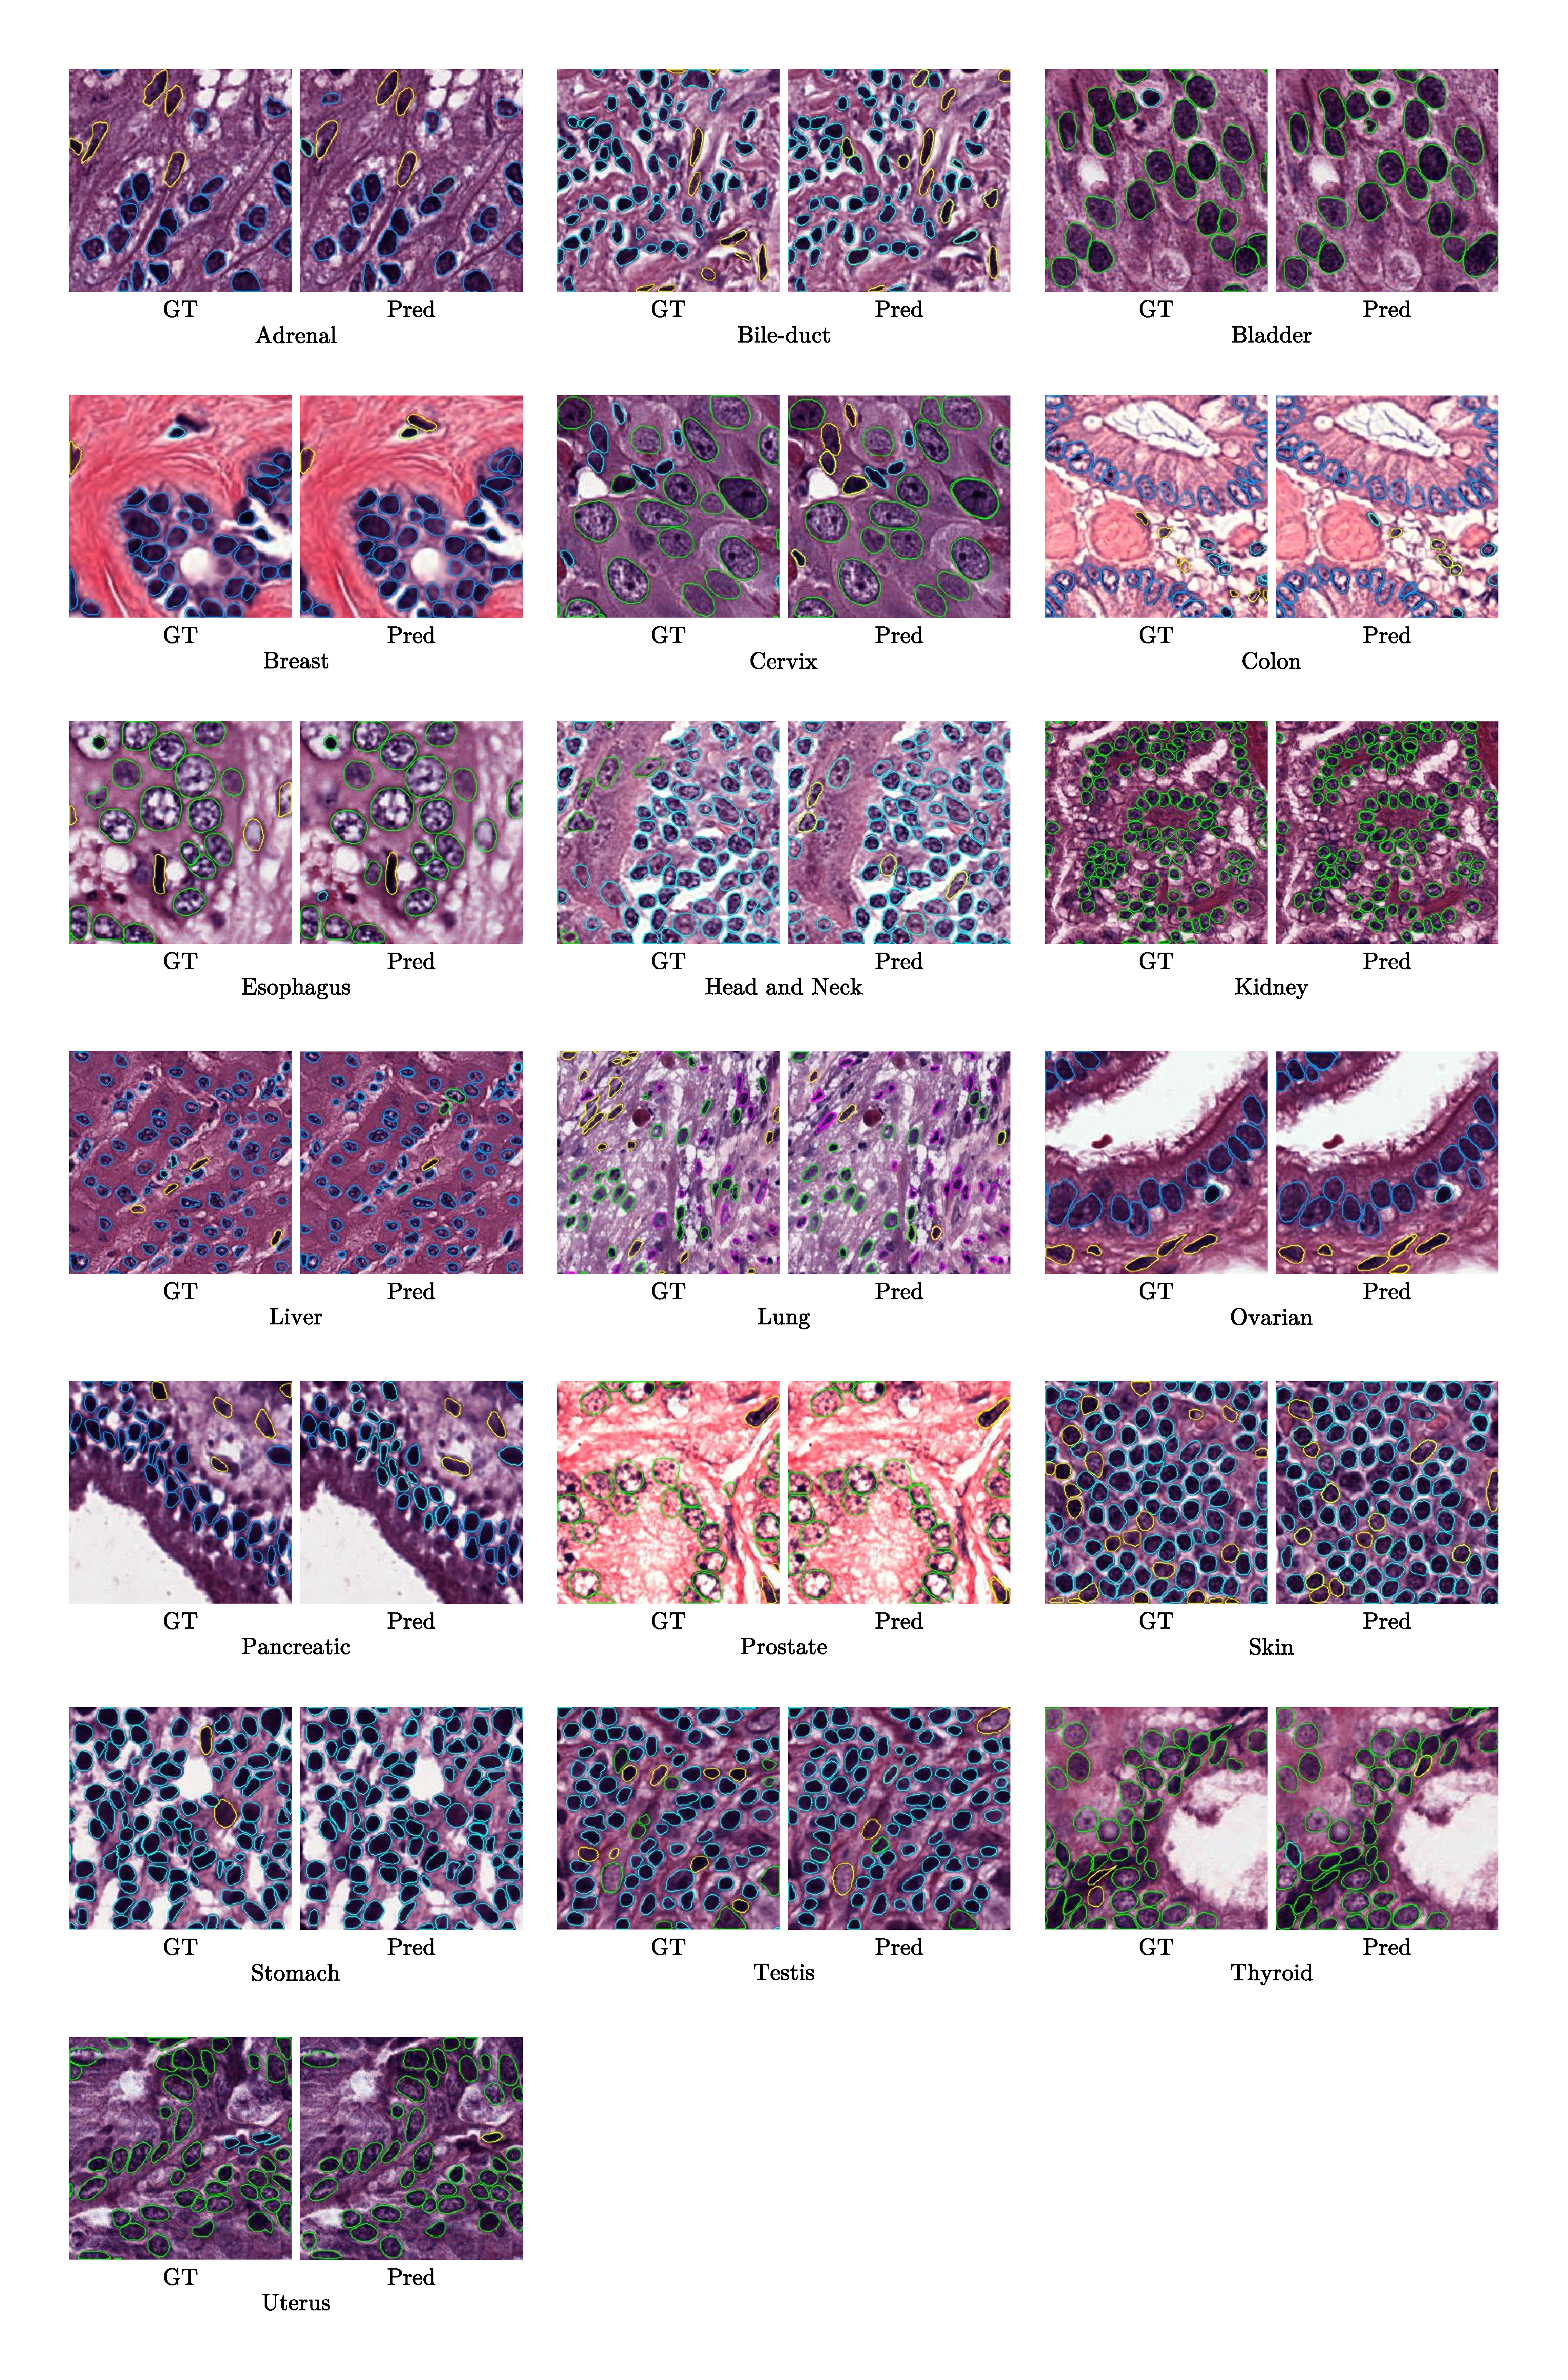
\includegraphics[width=\textwidth]{contents/chapter-4/fig/visual-tissue.pdf}
	\caption{RayCastED-B predictions across the 19 PanNuke tissue types.}
	\label{fig:visual-tissue}
\end{figure}

\begin{table}[H]
	\centering
	\caption{Per-nuclei-type precision, recall, and F1-score on the PanNuke test set. Nuclei types follow the PanNuke five-class taxonomy. CellPose-SAM does not provide nuclei classification. The best value in each column is shown in \textbf{bold}.}
	\label{tab:per-type}
	\small
	\resizebox{\textwidth}{!}{%
	\begin{tabular}{l>{\columncolor{blue!7}}c >{\columncolor{green!7}}c >{\columncolor{gray!10}}c >{\columncolor{blue!7}}c >{\columncolor{green!7}}c >{\columncolor{gray!10}}c >{\columncolor{blue!7}}c >{\columncolor{green!7}}c >{\columncolor{gray!10}}c >{\columncolor{blue!7}}c >{\columncolor{green!7}}c >{\columncolor{gray!10}}c >{\columncolor{blue!7}}c >{\columncolor{green!7}}c >{\columncolor{gray!10}}c}
		\hline
		& \multicolumn{3}{c}{\textbf{Neoplastic}} & \multicolumn{3}{c}{\textbf{Inflammatory}} & \multicolumn{3}{c}{\textbf{Connective}} & \multicolumn{3}{c}{\textbf{Necrosis}} & \multicolumn{3}{c}{\textbf{Epithelial}} \\
		\textbf{Method} & \textbf{P} & \textbf{R} & \textbf{F1} & \textbf{P} & \textbf{R} & \textbf{F1} & \textbf{P} & \textbf{R} & \textbf{F1} & \textbf{P} & \textbf{R} & \textbf{F1} & \textbf{P} & \textbf{R} & \textbf{F1} \\
		\hline
		StarDist      & 0.6213 & 0.5998 & 0.6104 & 0.5857 & 0.5431 & 0.5636 & 0.5719 & 0.4009 & 0.4714 & 0.3333 & 0.0009 & 0.0019 & 0.4326 & 0.2998 & 0.3541 \\
		CellPose-SAM  & -- & -- & -- & -- & -- & -- & -- & -- & -- & -- & -- & -- & -- & -- & -- \\
		LKCell        & 0.7285 & \textbf{0.7167} & \textbf{0.7225} & \textbf{0.7090} & \textbf{0.6603} & \textbf{0.6838} & 0.6067 & \textbf{0.6002} & \textbf{0.6034} & 0.4497 & 0.3340 & 0.3833 & 0.7019 & \textbf{0.7459} & 0.7232 \\
		HoVer-NeXt    & \textbf{0.7372} & 0.6566 & 0.6946 & 0.6932 & 0.6392 & 0.6651 & \textbf{0.6207} & 0.5722 & 0.5955 & \textbf{0.4750} & 0.3595 & \textbf{0.4093} & \textbf{0.7630} & 0.6909 & \textbf{0.7252} \\
		RayCastED-S   & 0.6775 & 0.6441 & 0.6604 & 0.5546 & 0.6009 & 0.5768 & 0.5105 & 0.5053 & 0.5079 & 0.3826 & \textbf{0.4062} & 0.3940 & 0.6000 & 0.6628 & 0.6298 \\
		RayCastED-B   & 0.6825 & 0.6718 & 0.6771 & 0.5751 & 0.5947 & 0.5848 & 0.5318 & 0.5322 & 0.5320 & 0.3919 & 0.3927 & 0.3923 & 0.6615 & 0.6534 & 0.6574 \\
		RayCastED-L   & 0.7329 & 0.6558 & 0.6922 & 0.6609 & 0.5907 & 0.6239 & 0.6029 & 0.5086 & 0.5518 & 0.4470 & 0.3532 & 0.3946 & 0.7339 & 0.6540 & 0.6916 \\
		\hline
	\end{tabular}%
	}
\end{table}


The per-type analysis shows LSP-DETR dominating across most nuclear categories, achieving the best F1 on Neoplastic (0.750), Inflammatory (0.697), Necrosis (0.474), and Epithelial (0.754). Two notable exceptions emerge where RayCastED holds an advantage. First, in the Necrosis category, RayCastED-S achieves the highest recall (0.486) -- remarkable for the smallest model in the comparison -- and the broader RayCastED family shows competitive recall on this rare minority class. Second, RayCastED-L achieves competitive F1 on Inflammatory (0.624) despite having an order of magnitude fewer parameters than LSP-DETR (9.44M vs.\ 45M) and LKCell (699.7M). HoVer-NeXt also claims two F1 wins (Necrosis 0.492 and Connective 0.646) using only an F1-trained variant, suggesting strong shape discrimination even without explicit precision/recall supervision.

\begin{table}[H]
	\centering
	\caption{Model complexity and time complexity benchmarking. Best overall is shown in \textbf{bold}.}
	\label{tab:benchmark-efficiency}
	\small
	\begin{tabular}{lccc}
		\hline
		\textbf{Method} & \textbf{Params} & \textbf{GFLOPs} & \textbf{Time Complexity} \\
		\hline
		StarDist      & 1.46M     & 8.14   & $O(n + k^2)$ \\
		CellPose-SAM  & $\sim$305M & 724   & $O(n^2)$ \\
		LKCell        & 163.8M    & 47.86  & $O(n \log n + kn)$ \\
		HoVer-NeXt    & 36M       & 24     & $O(n \log n + kn)$ \\
		RayCastED-S   & \textbf{0.81M}  & \textbf{1.38}  & $O(n)$ \\
		RayCastED-B   & 2.6M      & 5.52   & $O(n)$ \\
		RayCastED-L   & 9.44M     & 12.42  & $O(n)$ \\
		\hline
	\end{tabular}
\end{table}


As shown in Table~\ref{tab:benchmark-efficiency}, the parameter and GFLOPs gaps between RayCastED and the baselines are substantial. LKCell sits at the heavy extreme with 699.7M parameters and 214 GFLOPs, while the other baselines (StarDist, CPP-Net, HoVer-NeXt, LSP-DETR) cluster in the 32--45M range with 24--35 GFLOPs. RayCastED-S, the lightest variant, is over $40\times$ smaller than the next-lightest baseline and almost $860\times$ smaller than LKCell, while RayCastED-L (9.44M) remains $3$--$5\times$ smaller than the baseline cluster. Critically, the entire RayCastED family shares the same $O(n)$ linear time complexity as LSP-DETR via its post-hoc-processing-free design: without NMS or watershed, inference scales proportionally to the number of anchor positions rather than the number of detected objects. Since the anchor grid is fixed by input resolution and stride, this complexity is image-size agnostic -- the model accepts arbitrarily sized inputs without a super-linear increase in cost, enabling throughput-consistent deployment across varying tile dimensions. The two NMS-based contour methods (StarDist, CPP-Net) incur $O(n+k^2)$ complexity from their per-instance post-processing, while LKCell and HoVer-NeXt pay $O(n \log n + kn)$ for their watershed-based instance separation.

\subsection{Generalization Test}
\label{sec:generalization}

To evaluate cross-dataset generalization without fine-tuning, we apply the PanNuke-trained RayCastED-B directly to
MoNuSAC, panopTILs, and PUMA. Table~\ref{tab:generalization} reports the zero-shot performance in terms of
bPQ, precision, recall, and F1.

\begin{table}[H]
	\centering
	\caption{Zero-shot generalization results. RayCastED-B is trained on PanNuke and evaluated on three unseen datasets without fine-tuning.}
	\label{tab:generalization}
	\small
	\begin{tabular}{lccccc}
		\hline
		\textbf{Dataset} & \textbf{AJI} & \textbf{bPQ} & \textbf{F1} & \textbf{P} & \textbf{R} \\
		\hline
		PUMA      & 0.6336 & 0.6463 & 0.7774 & 0.7579 & 0.7979 \\
		panopTILs & 0.2673 & 0.2554 & 0.5057 & 0.3683 & 0.8063 \\
		MoNuSAC   & 0.3478 & 0.2648 & 0.5636 & 0.5907 & 0.5390 \\
		\hline
	\end{tabular}
\end{table}


RayCastED-B generalizes well to PUMA, achieving performance comparable to the in-domain PanNuke results. For panopTILs and MoNuSAC, however, the zero-shot performance indicates that domain-specific retraining is necessary to bridge the distribution gap. In general, fine-tuning or retraining RayCastED on the target dataset is recommended for optimal performance in a new clinical domain.

\section{Edge Deployment Evaluation}
\label{sec:edge-deployment}

\begin{figure}[H]
	\centering
	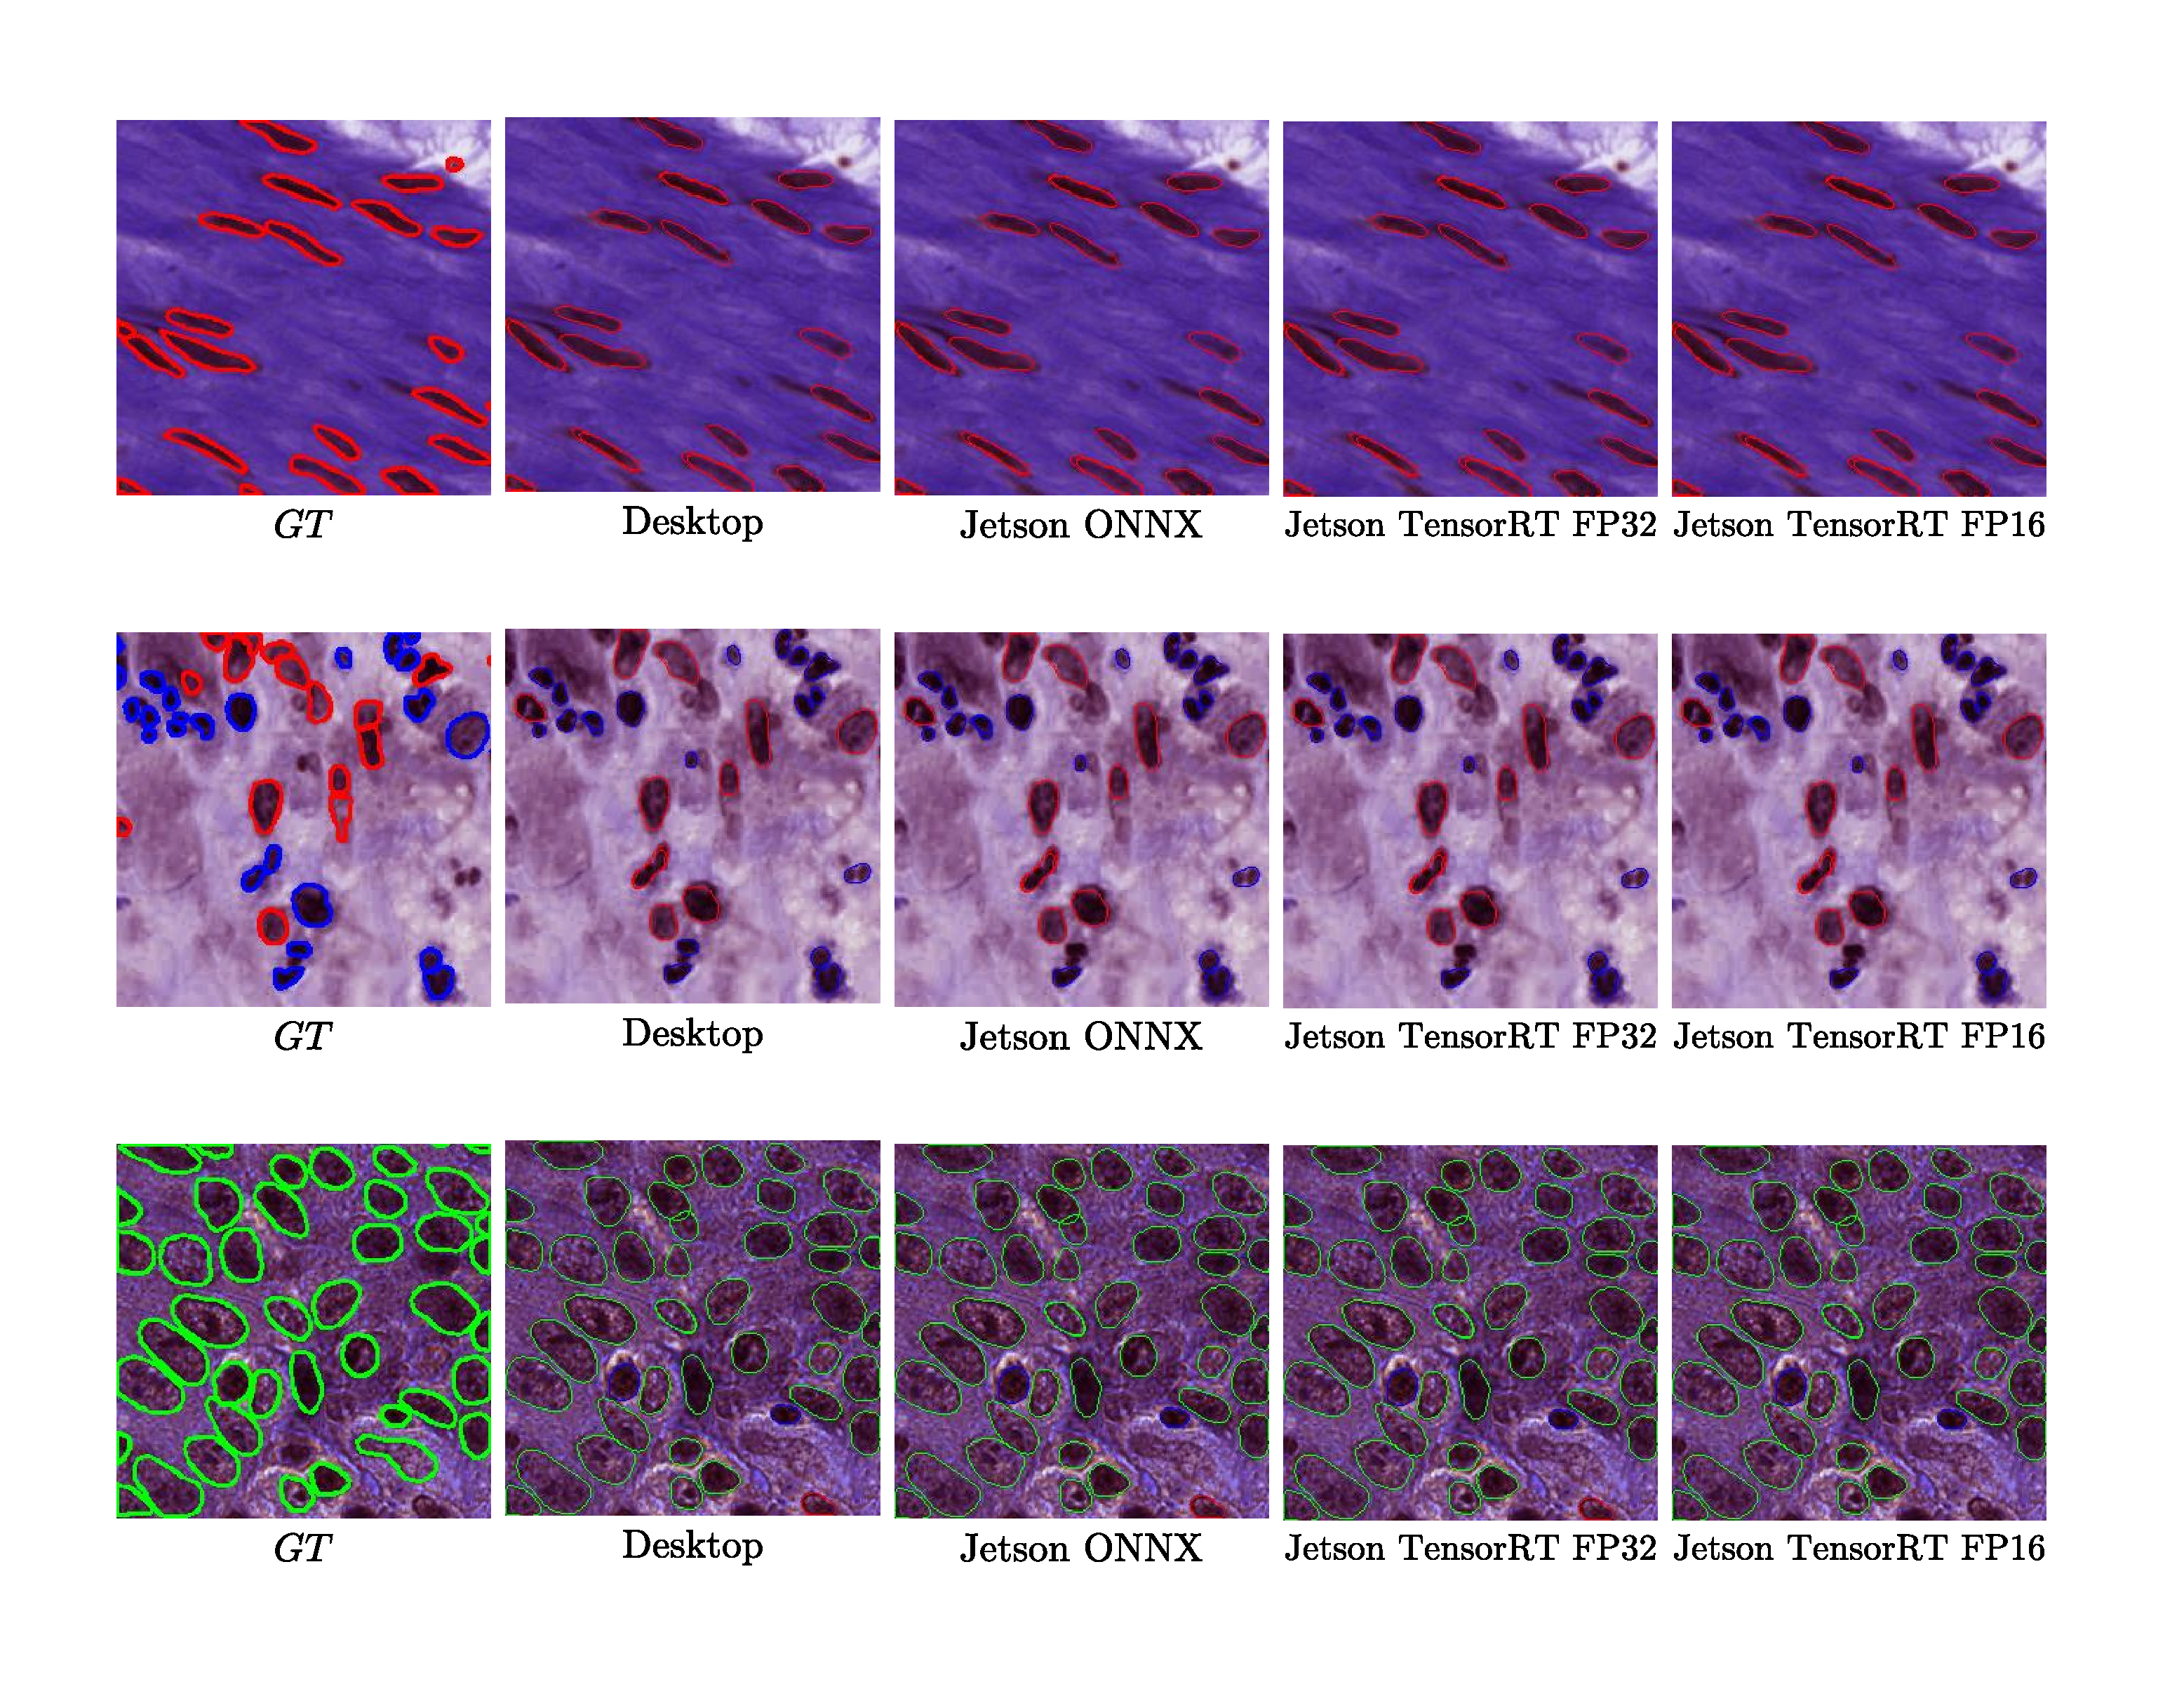
\includegraphics[width=\textwidth]{contents/chapter-4/fig/visual-edge.pdf}
	\caption{Comparison of edge deployment output across platforms.}
	\label{fig:visual-edge}
\end{figure}

To assess the practicality of RayCastED for clinical deployment on resource-constrained hardware, we benchmark the
smallest variant (RayCastED-S) on two platforms: a desktop GPU (RTX 5070 Ti) and an embedded AI accelerator
(Jetson Orin Nano). Table~\ref{tab:edge} compares accuracy and throughput across five configurations.

\begin{table}[H]
	\centering
	\caption{Edge deployment evaluation of RayCastED-B across GPU and embedded platforms. All measurements are taken over the PanNuke test set with batch size 1. The best value in each column is shown in \textbf{bold}.}
	\label{tab:edge}
	\small
	\resizebox{\textwidth}{!}{%
	\begin{tabular}{lccccccc}
		\hline
		\textbf{Configuration} & \textbf{bPQ} & \textbf{mPQ} & \textbf{F1} & \textbf{Precision} & \textbf{Recall} & \textbf{Predicted Nuclei} & \textbf{Runtime (ms)} \\
		\hline
		RTX 5070 Ti, PyTorch           & 0.6024 & 0.4526 & 0.7409 & 0.7419 & 0.7400 & \textbf{65679 / 65847} & 3.59 \\
		RTX 5070 Ti, TensorRT          & 0.6003 & 0.4735 & 0.7745 & 0.8067 & \textbf{0.7448} & 60796 / 65847 & \textbf{2.70} \\
		Jetson Orin Nano, ONNX         & 0.5986 & 0.4763 & 0.7748 & 0.8169 & 0.7368 & --            & 88.2 \\
		Jetson Orin Nano, TF32         & \textbf{0.6118} & \textbf{0.4897} & 0.7749 & \textbf{0.8170} & 0.7369 & 59394 / 65848 & 38.1 \\
		Jetson Orin Nano, FP16         & 0.6112 & 0.4894 & \textbf{0.7753} & 0.8140 & 0.7401 & --            & 29.2 \\
		RTX 2080 Super, TensorRT       & 0.5983 & 0.4746 & 0.7746 & 0.8149 & 0.7381 & 59640 / 65848 & 38.8 \\
		\hline
	\end{tabular}%
	}
\end{table}


The PyTorch baseline on the RTX 5070 Ti achieves near-exact predicted nuclei counts, confirming that the end-to-end inference pipeline operates correctly. When compiled with TensorRT, the RTX 5070 Ti reaches a per-image latency of 2.70~ms, representing a substantial speedup over PyTorch. Unexpectedly, TensorRT deployment on the Jetson Orin Nano yields consistently higher bPQ and mPQ than the desktop GPU across both FP16 and TF32 configurations. This is unlikely to stem from reduced precision, since TF32 and FP16 produce near-identical metrics. A plausible explanation is that TensorRT's aggressive graph-level optimizations for the Jetson target architecture restructure the operator execution order in a way that benefits the model numerically. The absence of such gains on the older RTX 2080 Super (similarly running TensorRT) supports the hypothesis that the effect is architecture-specific rather than a universal property of engine compilation.

\section{Ablation Study}
\label{sec:ablation}

To isolate the contribution of key design choices, we conduct two controlled experiments using
RayCastED-B as the base configuration.

\subsection{Study on Number of Rays}
\label{sec:ablation-rays}

We vary the number of rays $R$ while keeping all other hyperparameters fixed, measuring
both detection accuracy and polygon fidelity. Table~\ref{tab:ablation-rays} reports the
results for $R \in \{8, 16, 32, 64\}$.

\input{contents/chapter-4/tab/ablation-rays}

Increasing the number of rays from $R=8$ to $R=64$ yields only modest overall performance improvement: bPQ rises from 0.5902 to 0.6024, while mPQ is non-monotonic, peaking at $R=16$ (0.4606) and then declining slightly at $R=32$ and $R=64$. The standard deviations across all ray configurations do not differ significantly, indicating that the ray count has minimal influence on prediction consistency. This behavior admits a simple explanation rooted in nuclear morphology.

The majority of nuclei in H\&E histopathology are approximately elliptical, a consequence of the convexity enforced by the nuclear lamina discussed in Section~\ref{sec:raycast-validation} and Section~\ref{sec:nuclear-morphology}. An elliptical target is well-approximated by a polygon with as few as eight rays, so the model learns to predict smooth elliptical envelopes regardless of the available angular resolution. Even at $R=64$, the network has the capacity to draw 64 independent rays but defaults to an ellipse-like shape because doing so already covers most of the nuclear area and achieves good overlap with the ground truth. This learned elliptical prior is sufficient for the common case but hurts on the minority of irregularly shaped nuclei (pleomorphic malignant cells, overlapping boundaries) where finer angular detail would actually help; the model cannot break out of its elliptical default to exploit the extra boundary resolution that denser rays offer.

Importantly, this is not a limitation of the representation itself. Section~\ref{sec:raycast-validation} (Table~\ref{tab:raycast-iou}) showed that increasing $R$ substantially improves the geometric mask IoU at the representation level, so the polygon parameterization is sound. The bottleneck is model capacity: RayCastED-B, at 2.6M parameters, is the smallest variant in the family and converges to the easy elliptical solution rather than learning the boundary-discrimination features that denser rays would require. A larger backbone could potentially exploit the higher angular resolution, leaving this as a direction for future work.

\subsection{Study on Different Wavelet}
\label{sec:ablation-wavelet}

We compare the Haar wavelet used in ResoConv against alternative wavelet families and a
strided-convolution baseline. Table~\ref{tab:ablation-wavelet} reports detection and
segmentation metrics for each configuration.

\begin{table}[H]
	\centering
	\caption{Ablation study on the wavelet transform used in ResoConv. All experiments use RayCastED-B with $R=64$. Best per column in \textbf{bold}.}
	\label{tab:ablation-wavelet}
	\small
	\begin{tabular}{lccccc}
		\hline
		\textbf{Wavelet} & \textbf{bPQ} & \textbf{mPQ} & \textbf{F1} & \textbf{Precision} & \textbf{Recall} \\
		\hline
		Haar (db1)         & \textbf{0.6024} & \textbf{0.4526} & \textbf{0.7409} & \textbf{0.7419} & \textbf{0.7400} \\
		Daubechies-2 (db2) & 0.6001 & 0.4435 & 0.7328 & 0.7269 & 0.7388 \\
		Daubechies-4 (db4) & 0.5905 & 0.4379 & 0.7148 & 0.7046 & 0.7252 \\
		\hline
	\end{tabular}
\end{table}


The best performance consistently comes from the Haar (db1) wavelet. Increasing the number of filter taps (db2, db4) introduces feature smoothing that attenuates the fine-grained edges, chromatin texture, and boundary transitions that distinguish individual nuclei. This smoothing removes discriminative high-frequency content essential for accurate detection and segmentation, resulting in regressed performance on all metrics.
